\section{Saving System State: Snapshots}

This section discusses saving state. This is useful for fault-tolerance and system migrations.

\begin{Def}[Snapshot]

    A \textbf{snapshot} is a consistent global state of a distributed system at a specific point in time. 
\end{Def}

\begin{Def}[Consistent vs. Inconsistent Snapshots]

    To evaluate a snapshot's consistency, we compare events in the system \textbf{pre-snapshot} (events before the snapshot) 
    and \textbf{post-snapshot} (events after the snapshot). The snapshot itself is instantaneous, like a photograph. 
    Given an event ordering $r$:
    
    \begin{itemize}
        \item \textbf{Consistent Snapshots}: Respect causal dependencies. Let there be events $e_1$ and $e_2$; If $e_1 \rightarrow_r e_2$, then $e_1$ must be included in the snapshot if $e_2$ is present.
        \item \textbf{Inconsistent Snapshots}: Violate causal dependencies. If $e_2$ is included without 
        the causally preceding event $e_1$, then the snapshot is inconsistent.
    \end{itemize}
\end{Def}

\vspace{-1em}
\begin{figure}[h]
    \centering
    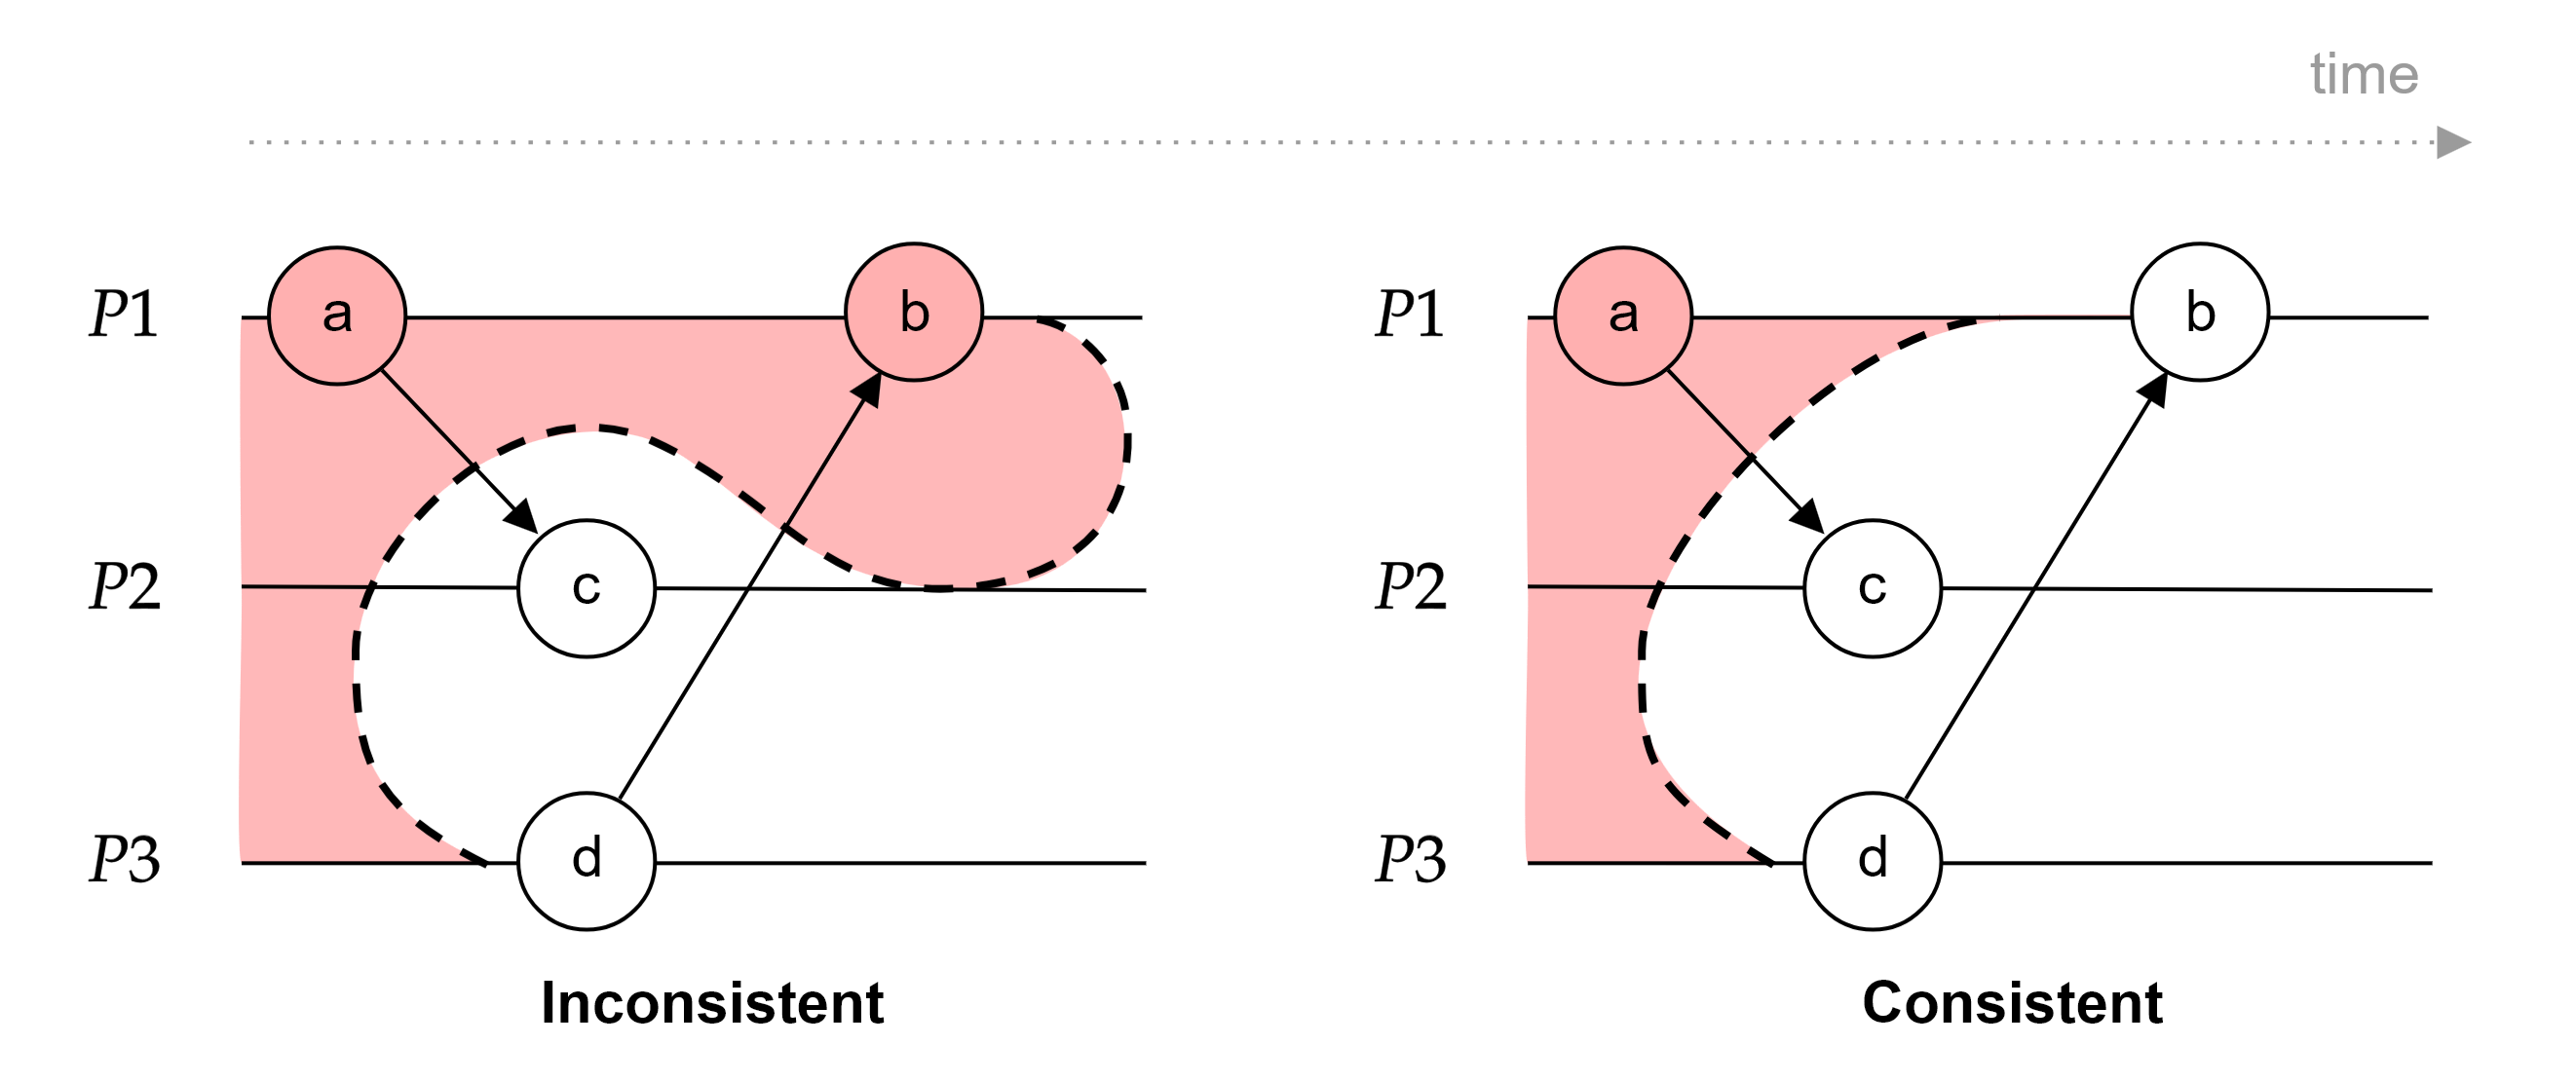
\includegraphics[width=.9\textwidth]{Sections/snap/snap.png}
    \caption{Inconsistent vs. Consistent Snapshots (pre-snapshot highlighted in red)}
\end{figure}

\noindent 
Here, in the inconsistent snapshot, $b$ is included without $d$, its causally preceding event. In the consistent snapshot, only $a$ is 
included. In this snapshot $c$ and $d$ could be added without violating causality.
